\documentclass{article}
\usepackage{tikz}
\usepackage[a4paper]{geometry}
\usepackage{fancyhdr}
\pagestyle{fancy}
\lhead{Nuklidkarten nutzen}
\rhead{März 2026}
\begin{document}
 
\newcommand{\karte}[4]{
 \foreach \i in {0,...,5} { 
  \draw (#1, \i*0.5) -- (#1+2.5, \i*0.5);
  \draw (#1+\i*0.5, 0) -- (#1+\i*0.5, 2.5);
 };
 \node[above left] at (#1, 2.5) {$Z$}; 
 \node[below right] at (#1+2.5, 0) {$N$};
 
 \node[below] at (#1+1.25, 0) {#2-Strahlung};
 
 \draw[thick, red, ->] (#1+1.25, 1.25) -- ({#1+1.25+(#3*0.5)}, {1.25+(#4*0.5)});
} 
 
\section{Nuklidkarten nutzen}
Nuklidkarten sind zweidimensionale Tabellen, welche entsprechend der Neutronenzahl $N$ auf der $x$-Achse und der Protonenzahl $Z$ auf der $y$-Achse unterschiedliche Nuklide darstellt.
 
Je nach Karte ist in der Regel der Name, die Zerfallsart, die Halbwertszeit und die Energie angegeben. Genaueres ist in der Legende der Karte geklärt.
 
\subsection{Zerfallsrichtungen}
Gemäß den konstanten Achsen und den bekannten Neutronen und Protonenzahlen der Emissionen der Zerfallsarten, kann jeder Zerfall als eine Art bewegung auf der Achse angesehen werden.
\begin{center} 
\begin{tikzpicture}
 \karte{0}{$\alpha$}{-2}{-2}
 \karte{4.5}{$\beta^+$}{1}{-1}
 \karte{9}{$\beta^-$}{-1}{1}
\end{tikzpicture}
\end{center}
Dies kann wiederholt werden, bis ein stabiles Nuklid gefunden wird, um eine Zerfallsreihe aufzustellen. 
 
\end{document}